Di dalam suatu komputer sudah pasti ada suatu mekanisme penyimpanan, contohnya
seperti memori utama yang dimiliki sistem seperti RAM (Random Access Memory).

\begin{figure}[h]
    \centering
    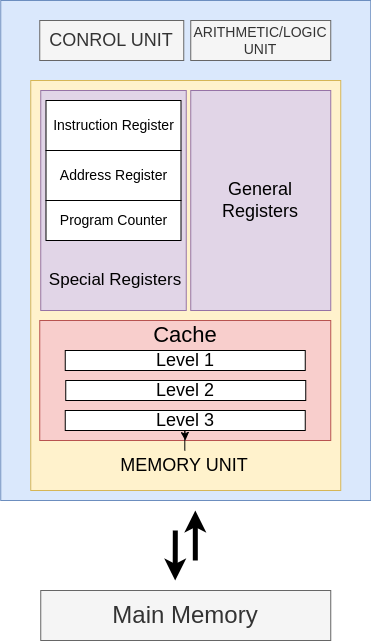
\includegraphics[scale=0.5]{MEMUNITDIAG}
    \caption{Diagram Unit Memori}
    \label{fig:MEMUNITDIAG}
\end{figure}

Namun selain RAM, CPU pun memiliki tempat penyimpanan tersendiri yang kecil didalam
chipset CPU itu sendiri, media penyimpanan tersebut disebut dengan Memory Unit.

Didalam suatu CPU, terdapat dua jenis Memory Unit yang kerap dijumpai,
yaitu Register dan juga System Cache atau CPU Cache.

Perbedaan antara Register dengan Sistem Cache terletak pada ukuran memori yang
dimiliki serta kegunaan yang mereka miliki. Berikut adalah penjelasannya.

\begin{enumerate}[label=\alph*.]

  \item \textbf{Register}

    Register adalah tempat-tempat penyimpanan yang relatif berukuran kecil,
    yang terletak di dalam chipset suatu CPU.

    Besarnya penyimpanan suatu register berbeda-beda tergantung dari
    arsitektur atau rancangan yang dimiliki CPU tersebut, namun pada
    umumnya akan berukuran diantara 8 bit dan 64 bit.

    Special Register adalah register-register yang memiliki fungsi khusus yang
    sudah ditetapkan oleh rancangan suatu CPU, maka register-register ini
    berkaitan erat dengan proses-proses yang berlangsung didalam suatu CPU.

    Selain Special Register, terdapat juga General Register atau General Purpose
    Register, General Purpose Register ini adalah register-register yang tidak
    memiliki fungsi khusus dan dapat digunakan secara bebas karena tidak terikat
    dengan proses CPU.

    Special Register memiliki beberapa tipe bedasarkan fungsi atau data yang
    ia simpan, berikut adalah tipe-tipenya.

    \begin{enumerate}[label=\roman*.]

      \item \textbf{Current Instruction Register (CIR/IR)}

        Register yang menyimpan alamat memori dari instruksi yang
        sedang diproses.

      \item \textbf{ Program Counter Register  (PC) }

        Register yang menyimpan alamat memori selanjutnya dari suatu instruksi
        yang akan dijalankan.

      \item \textbf{Accumulator (AC)}

        Register yang menyimpan informasi terakhir dari suatu data yang diakses
        dari memori.

      \item \textbf{Memory Address Register (MAR)}

        Register yang menyimpan alamat memori yang dapat diakses jika diperlukan.

      \item \textbf{Memory Data Register (MDR) dan Memory Buffer Register (MBR)}

        Register yang menyimpan data yang akan di akses atau dikirim ke memori.

      \item \textbf{Condition Code Register}

        Register yang menyimpan status akhir dari suatu operasi.

      \item \textbf{Temporary Register}

        Register yang hanya menyimpan data-data sementara.

      \item \textbf{Input Register}

        Register yang menyimpan sebuah karakter dari input.

      \item \textbf{Input Register}

        Register yang menyimpan sebuah karakter dari ouput.

      \item \textbf{Index Register (BX)}

        Register ini menyimpan nilai dari suatu alamat memori dan merubahnya
        menjadi alamat efektif untuk digunakan dalam merubah suatu alamat dari
        data yang di operasikan.

      \item \textbf{Stack Control Registers (SCR)}

        Suatu set memori register yang berbentuk tumpukan atau \textit{stack},
        yang dalam mengakses menggunakan metode LIFO atau Last in First Out, yang
        artinya data yang pertama kali di tambahkan atau berada di tumpukan paling
        bawah hanya bisa diakses setelah telah mengakses terlebih dahulu data
        yang berada diatasnya.

      \item \textbf{Flag Register (FR)}

        Suatu set Register yang menyimpan suatu keadaan (\textit{Flag}) suatu kondisi,
        biasanya berukuran 8 bytes dengan tiap kondisi digambarkan dengan data
        atau susunan bit berukuran 8 bit.

        Ada beberapa jenis keadaan yang disimpan, antara lain, \textit{Zero flags},
        \textit{Carry flag}, \textit{Parity flag}, \textit{Sign flag}, dan \textit{Overflow flag}

      \item \textbf{Segment Register (SR)}

        Menyimpan alamat suatu memori

      \item \textbf{Data Register (DX)}

        Menyimpan alamat suatu memori suatu data yang akan dioperasikan

    \end{enumerate}

  \item \textbf{System Cache}

    System Cache atau CPU Cache berfungsi untuk yang mempercepat proses
    pembacaan atau pengaksesan data dari memori utama (RAM) oleh CPU.

    Umumnya terdapat tiga tingkatan cache,
    yaitu L1 atau cache level 1 hingga ke L3 atau cache level 3.

    Bedasarkan Ensiklopedia Britannica, Cache atau Cache Memory adalah
    ``Memori tambahan yang secara sementara menyimpan instruksi dan data yang
    sering diakses agar dapat diproses lebih cepat oleh Central Processing Unit
    (CPU)``.

\end{enumerate}
